%Nama Kelompok: Sistem_Operasi_Deadlock
%Kelas: D4 TI 1B
%Alit Fajar Kurniawan(1174057) 
%Muhammad Iqbal Panggabean(1174063)
%Muhammad Afra Faris(1174041)
%Khadijah Hasanah Puteri Harahap(1174044)

\section {USB TO SERIAL}

\subsection {Pengertian USB}
\subsubsection {Apa itu USB ?}
	Universal Serial Bus atau yang disingkat dengan USB adalah sebuah teknologi yang dapat memungkinkan para penggunanya untuk dapat menghubungkan hardware eksternal contohnya seperti printer, keyboard, harddisk, flashdisk dan perangkat keras lainnya. kecepatan trnasfer data yang didukung oleh USB sebesar 12 Mbps. pada saat ini semua PC sudah memiliki port USB sendiri minimal 2 buah port USB.

\subsection {Ada Beberapa Keistimewaan dari USB}
\begin {enumerate}
\item
1. PC atau komputer dapat dijadikan sebagai sebuah host
\item
2. 127 perangkat atu lebih dapat terhubung ke PC atau komputer dengan menggunkan hub USb secara langsung
\item
3. Jika menggunakan kabel USB secara langsung hanya bisa mencapai 5 meter dan apabila menggunakan perangkat hub dapat sampai 30 meter jangkauannya
\item
4. Sifat perangkat USB 'hot swappable' yang artinya apabila ada perangkat keras yang telah menggunakan port USB sifatnya plug and play
\end {enumerate}

\subsection {Cara menghubungkan USB flash disk dengan komputer}
	USB port digunakan oleh flash disk denga tujuan untuk dapat mnghubungkan dengan komputer. fungsi dari flash disk itu sendiri yaitu untuk dapat menyimpan data dan flash disk juga memiliki batas maksimal penyimpanan. Mempelajari tentang bagaimana cara menghubungkan flash disk dengan komputer merupakan hal yang sangat mudah karena kita hanya memasukkan flash disk kedalam port USB yang tersedia di PC atau komputer. Ini merupakan salah satu cara komunikasi antara komputer atau PC dengan hardware yng dihubungkan dengan komputer atau PC dan dilakukan melalui USB To Serial.
	
	\begin{figure}[ht]
	\centerline{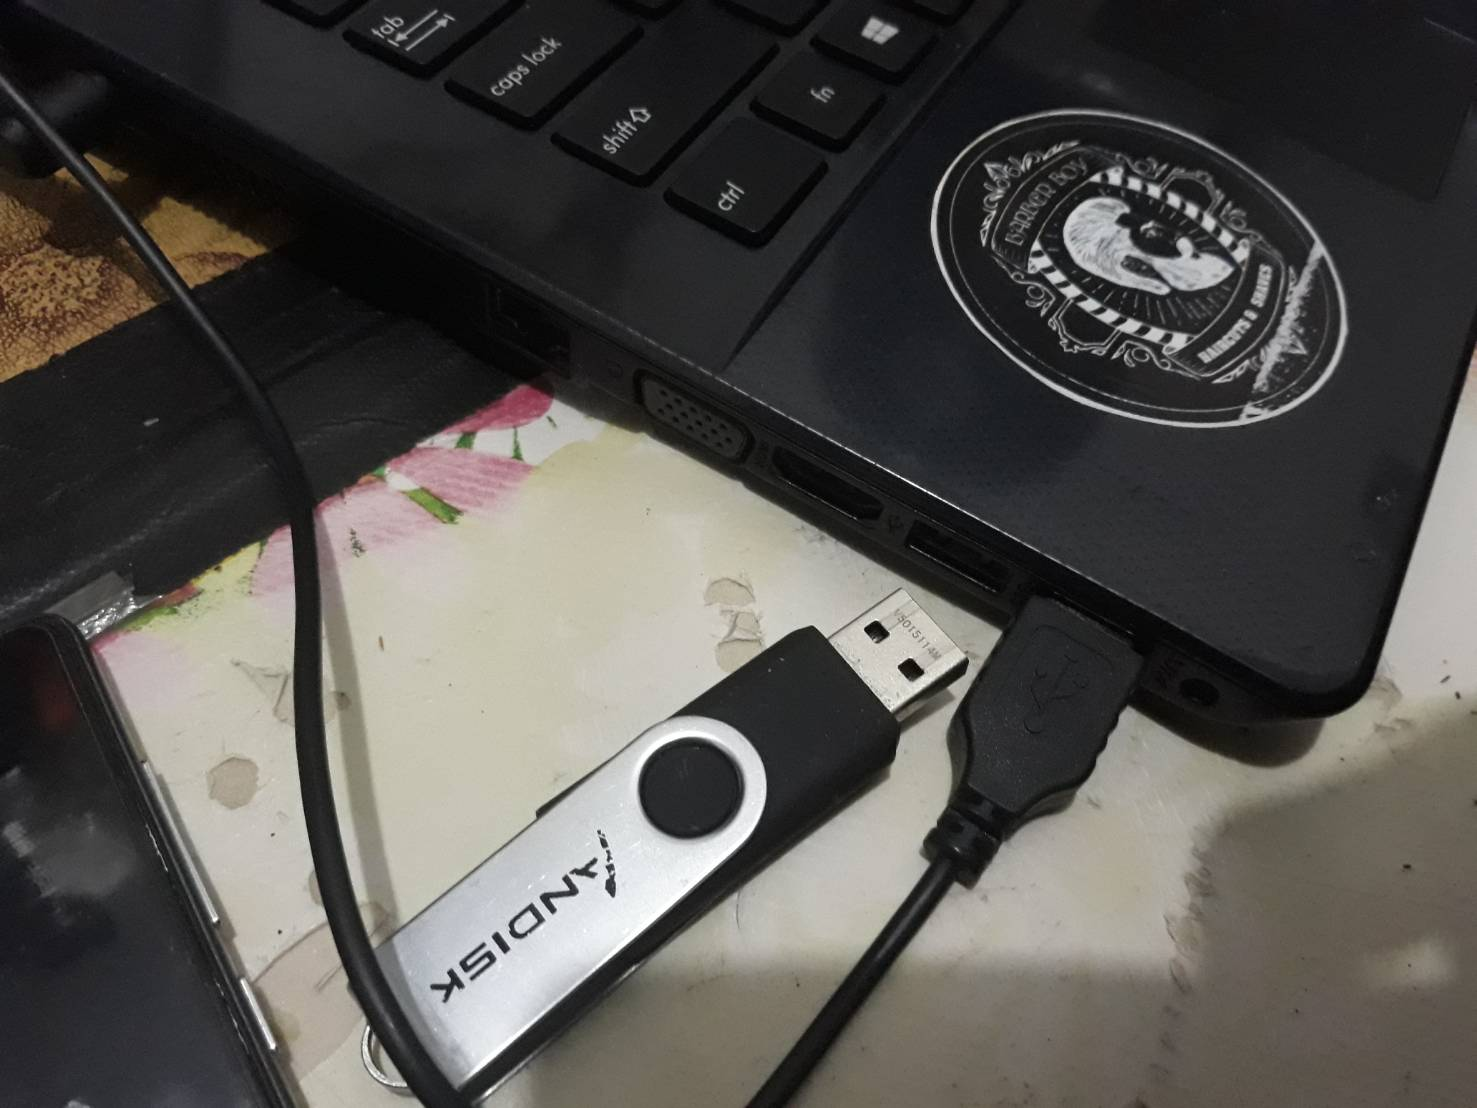
\includegraphics[width=1\textwidth]{figures/usb1.jpg}}
	\caption{Gambar memasukkan flash disk kedalam port usb pada PC}
	\label{Gambar}
	\end{figure}
      
      Gambar \ref{Gambar} Contoh gambar memasukkan flash disk kedalam port usb pada PC.

